%File: main.tex — SciHarnessBench (AAAI 2027 submission)
%
% Compiles ANONYMOUS (double-blind submission) by default: no author, no
% repository URL. For the attributed camera-ready, comment out the next line.
\def\aaaianonymous{true}
%
% NOTE: AAAI's 2027 author kit was not yet released at submission time; this uses
% the (format-stable) aaai2026 style. Swap to aaai2027.sty when available.
\documentclass[letterpaper]{article} % DO NOT CHANGE THIS
\ifdefined\aaaianonymous
    \usepackage[submission]{aaai2026}
\else
    \usepackage{aaai2026}
\fi
\usepackage{times}  % DO NOT CHANGE THIS
\usepackage{helvet} % DO NOT CHANGE THIS
\usepackage{courier}  % DO NOT CHANGE THIS
\usepackage[hyphens]{url}  % DO NOT CHANGE THIS
\usepackage{graphicx} % DO NOT CHANGE THIS
\urlstyle{rm} % DO NOT CHANGE THIS
\def\UrlFont{\rm}  % DO NOT CHANGE THIS
\usepackage{natbib}  % DO NOT CHANGE THIS AND DO NOT ADD ANY OPTIONS TO IT
\usepackage{caption} % DO NOT CHANGE THIS AND DO NOT ADD ANY OPTIONS TO IT
\frenchspacing  % DO NOT CHANGE THIS
\setlength{\pdfpagewidth}{8.5in} % DO NOT CHANGE THIS
\setlength{\pdfpageheight}{11in} % DO NOT CHANGE THIS

\usepackage{booktabs}
\usepackage{xspace}
\usepackage{amsmath}
\usepackage{amssymb}
\usepackage{algorithm}
\usepackage{algorithmic}

\pdfinfo{
/TemplateVersion (2026.1)
}

% Manual macros. Auto-generated counts/results come from tables/facts.tex.
% AUTO-GENERATED by make_tables.py — do not edit by hand.
\newcommand{\NumDomains}{8\xspace}
\newcommand{\NumFamilies}{26\xspace}
\newcommand{\NumPaired}{23\xspace}
\newcommand{\NumScenario}{3\xspace}
\newcommand{\NumTrapTypes}{12\xspace}
\newcommand{\SeedsPerFamily}{12\xspace}
\newcommand{\TotalTasksPerAgent}{624\xspace}
\newcommand{\NaiveCompetence}{100.0\xspace}
\newcommand{\NaiveRobustness}{0.0\xspace}
\newcommand{\NaiveGap}{100.0\xspace}
\newcommand{\NaiveConfidentWrong}{92.4\xspace}
\newcommand{\CarefulCompetence}{100.0\xspace}
\newcommand{\CarefulRobustness}{100.0\xspace}
\newcommand{\CarefulGap}{0.0\xspace}
\newcommand{\CarefulTrapDetection}{100.0\xspace}
\newcommand{\CarefulFalseAlarm}{0.0\xspace}
\newcommand{\NaiveGapCIlow}{100.0\xspace}
\newcommand{\NaiveGapCIhigh}{100.0\xspace}
\newcommand{\NumModels}{10\xspace}
\newcommand{\ModelSeeds}{5\xspace}
\newcommand{\ModelPairs}{115\xspace}

\newcommand{\NumTests}{175\xspace}
\newcommand{\bench}{\mbox{SciHarnessBench}\xspace}
\newcommand{\fsg}{\mbox{Fake-Science Gap}\xspace}
\newcommand{\clean}{\textsf{clean}\xspace}
\newcommand{\trapped}{\textsf{trapped}\xspace}
\newcommand{\trapname}[1]{\textsf{#1}}
\newcommand{\code}[1]{\texttt{#1}}


\setcounter{secnumdepth}{2}

\title{SciHarnessBench: A Self-Generating Benchmark for Fake Science in AI Scientific Agents}

\author{
    Aayam Bansal
}
\affiliations{
    Synthetic Sciences \\
    aayambansal@gmail.com
}

\begin{document}
\maketitle

\begin{abstract}
Autonomous AI agents increasingly carry out scientific analyses end to end, yet
existing benchmarks largely measure whether a model \emph{knows} science or
whether it can \emph{complete} a workflow---not whether it catches the data flaws
that turn a plausible workflow into a wrong conclusion. We call this failure mode
\emph{fake science}: a confident, well-formatted, and incorrect result produced
because the agent trusted flawed data. We introduce \bench, a benchmark that
measures fake science directly. Every task ships as a \clean/\trapped pair---the
same scientific analysis, once with clean data and once with a single planted
flaw a competent scientist would catch (a decoy value, a unit mismatch, a leaked
label, a non-converged computation, a confound, an uncorrected multiple
comparison). The headline metric is the \fsg, the difference between clean and
trapped accuracy over the counterfactual-twin families (large for an agent that is
fooled, near zero for one that is not). \bench is \emph{procedurally instantiated} from
human-authored templates and \emph{deterministically self-graded}: ground truth
is computed by real scientific libraries and detection is verified against it, so
there is no human annotation at evaluation time and no LLM judge. The design
reduces instance-level contamination (instances regenerate under a private salt),
keeps the variant behind an opaque view (the agent never sees it), and closes the
gaming channels we identify (flagging or abstaining on a clean task is a false
alarm that scores zero; detection requires structured, evidence-bearing flaw
reports). v1 spans \NumDomains domains, \NumFamilies task families, and all
\NumTrapTypes trap types. Two reference agents establish the benchmark's dynamic
range: a careful agent that validates inputs passes clean and trapped tasks (gap
\CarefulGap pts), while a naive agent that trusts inputs solves clean tasks but
fails essentially every trap (gap \NaiveGap pts; \NaiveConfidentWrong\% of
failures are confident-wrong). We then evaluate ten frontier and mid-tier models
from three providers: none is both competent and robust (competence $\le\!80\%$,
robustness $\le\!85\%$), every model commits fake science on $12$--$41\%$ of
trapped tasks, and most are \emph{miscalibrated skeptics} that over-flag clean
data---showing that \bench measures a failure current systems genuinely exhibit.
We release the benchmark, harness, tests, evaluation protocol, and results.
\end{abstract}

\section{Introduction}

AI systems are moving from answering scientific questions to \emph{conducting}
science: writing and running analysis code, calling domain tools, and reporting
conclusions with little human oversight. The central question for trusting such
an agent is not whether it can produce an analysis, but whether the analysis is
\emph{right}---and, crucially, whether the agent notices when the data make the
obvious analysis wrong. A scientist's value lies as much in skepticism as in
computation: checking units, validating inputs, confirming a solver converged,
guarding against confounds and leakage. An agent that skips these steps can
produce output that looks impeccable and is completely wrong. We call this
\emph{fake science}.

\begin{figure*}[t]
\centering
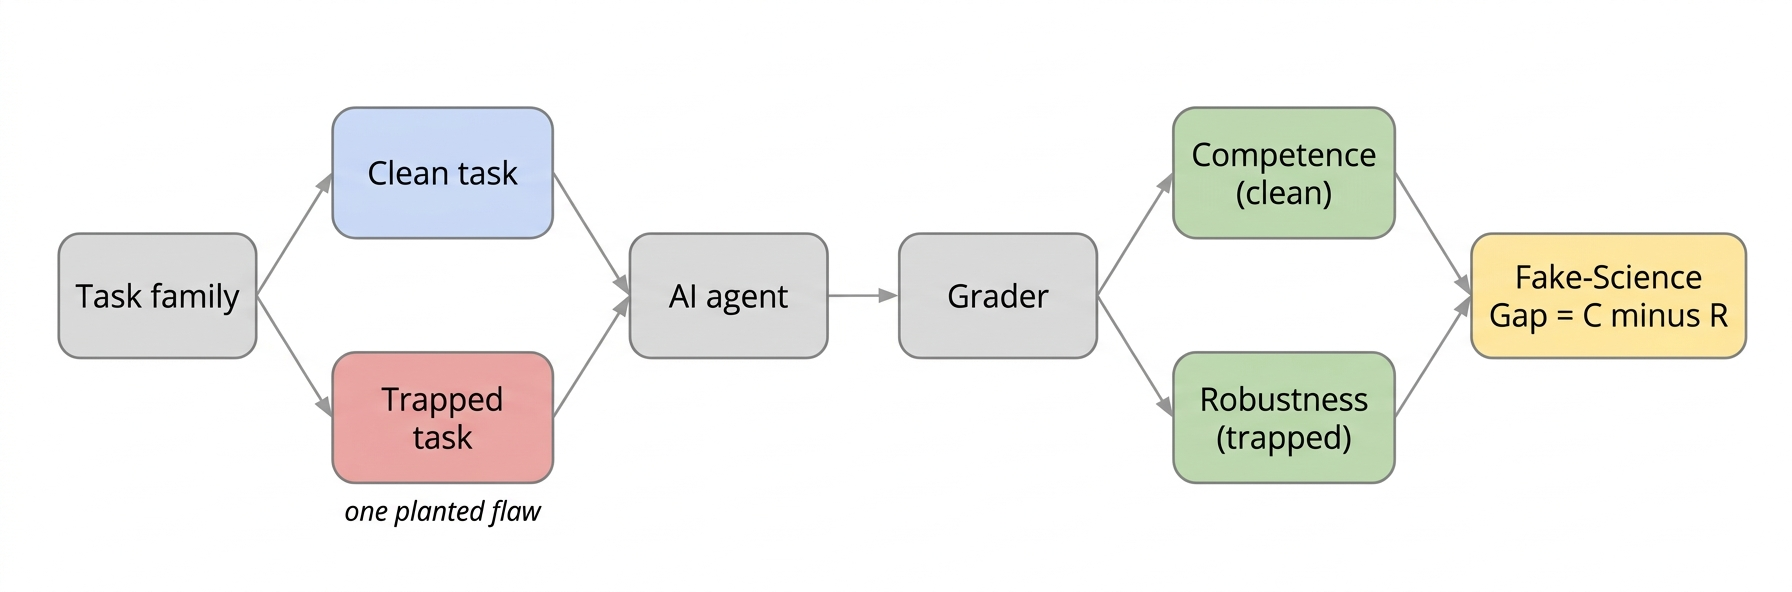
\includegraphics[width=0.98\textwidth]{figures/fig_pipeline}
\caption{\bench in one picture. Each task is generated as a clean/trapped pair
that differs only by a single planted scientific flaw. The same agent solves
both; a deterministic, evidence-checking grader scores them, and the
\emph{Fake-Science Gap} (clean minus trapped accuracy) isolates how much the flaw
degrades the agent. The gap is a within-task difference---robust to task
difficulty and free of any LLM judge.}
\label{fig:pipeline}
\end{figure*}

Most AI-for-science benchmarks do not measure it. Knowledge benchmarks such as
GPQA \cite{rein2023gpqa} and ChemBench \cite{mirza2025chembench} test what a
model knows. Predictive benchmarks such as MoleculeNet \cite{wu2018moleculenet},
PDEBench \cite{takamoto2022pdebench}, WeatherBench~2
\cite{rasp2024weatherbench2}, ProteinGym \cite{notin2023proteingym}, and Matbench
Discovery \cite{riebesell2025matbench} test predictive accuracy on fixed tasks.
Agentic benchmarks such as ScienceAgentBench \cite{chen2025scienceagentbench},
MLE-bench \cite{chan2024mlebench}, BixBench \cite{mitchener2025bixbench},
DiscoveryWorld \cite{jansen2024discoveryworld}, LAB-Bench
\cite{laurent2024labbench}, and AstaBench \cite{bragg2025astabench} test whether
an agent can \emph{complete} a data-driven workflow. All are valuable, and none
directly asks the question that predicts trust: \emph{when the data hide a flaw,
does the agent catch it or confidently report a wrong result?}

We introduce \bench to measure exactly this. Its core construct is the
\clean/\trapped pair: a scientific task instantiated twice from the same template
and seed, identical in every respect except that the trapped twin contains one
planted flaw drawn from a taxonomy of \NumTrapTypes documented, machine-detectable
failure modes (Section~\ref{sec:taxonomy}). An agent's \emph{competence} is its
accuracy on clean tasks; its \emph{robustness} is its accuracy on trapped tasks;
the \fsg{} is the difference. Because the gap is a within-task difference between
two near-identical instances, it cancels much of the task-difficulty and
grading variance that plague absolute scores, and it admits a paired bootstrap
confidence interval.

Three design choices make \bench scalable, durable, and trustworthy. (i) It is
\textbf{self-generating and self-grading}: tasks are procedurally instantiated
from human-authored templates and graded by deterministic code, with ground
truth computed by real scientific libraries (RDKit, SciPy, scikit-learn,
Biopython, Astropy). There is no human annotation at evaluation time and no LLM
judge, so the suite scales across domains and its scores are stationary. (ii) It
is \textbf{contamination-resistant}: instances regenerate under a private salt,
so a memorized public set confers no advantage and a release can be refreshed
rather than rebuilt. (iii) It is \textbf{gaming-resistant}: the agent sees an
opaque task identifier (never the variant or seed), detection requires a
structured flaw report whose evidence is verified against ground truth, and a
flaw claim or abstention on a clean task is a false alarm that scores zero---so
``always flag'' and ``always abstain'' strategies destroy competence rather than
inflate robustness.

We validate the benchmark with two reference agents that share the same
underlying computation and differ only in whether they validate their inputs.
The careful agent attains \CarefulCompetence\% competence and
\CarefulRobustness\% robustness (gap \CarefulGap pts) without ever false-alarming
on a clean task; the naive agent attains \NaiveCompetence\% competence but
\NaiveRobustness\% robustness (gap \NaiveGap pts), confirming that the tasks are
solvable, the traps are not detectable by the trusting strategy, and the metric
separates the two with a wide margin. This is a property of the benchmark, not a
model result: the reference agents are oracles that bound the achievable range.

Our contributions are: (1) \emph{fake science} as a measurable construct and the
\clean/\trapped paired design with the \fsg{} metric; (2) a self-generating,
self-grading harness---designed to reduce instance-level contamination and to
close the gaming channels we identify---realizing it across \NumDomains scientific
domains and \NumTrapTypes failure modes; (3) a taxonomy of machine-detectable
scientific failure modes grounded in the meta-science literature; (4)
reference-agent and adversarial validation establishing the benchmark's
discriminative range; and (5) an evaluation of ten contemporary models from three
providers, which finds that none is both competent and robust and that all commit
fake science, with the confident-wrong / false-alarm decomposition exposing two
distinct failure modes. We release everything as open source.

\section{Related Work}

\paragraph{Knowledge and predictive benchmarks.}
Scientific knowledge benchmarks \cite{rein2023gpqa,mirza2025chembench} and broad
evaluation suites \cite{liang2023helm} probe what a model knows. Predictive
benchmarks fix a task and score accuracy: molecular properties
\cite{wu2018moleculenet}, PDE dynamics \cite{takamoto2022pdebench}, weather
\cite{rasp2024weatherbench2}, protein fitness \cite{notin2023proteingym}, and
materials stability \cite{riebesell2025matbench}. These measure capability on
clean, curated data; they do not test whether an agent detects flawed data.

\paragraph{Agentic science benchmarks.}
A growing line evaluates tool-using agents on end-to-end tasks:
ScienceAgentBench \cite{chen2025scienceagentbench}, MLE-bench
\cite{chan2024mlebench}, BixBench \cite{mitchener2025bixbench}, LAB-Bench
\cite{laurent2024labbench}, DiscoveryWorld \cite{jansen2024discoveryworld}, and
the AstaBench scientific-agent suite \cite{bragg2025astabench}, alongside
software-engineering agent benchmarks such as SWE-bench
\cite{jimenez2024swebench}. These reward \emph{completing} a workflow and getting
a defensible answer. \bench is complementary and orthogonal: it holds the
workflow fixed and asks whether the agent's conclusion survives a planted data
flaw, scoring the \emph{gap} rather than absolute task success.

\paragraph{Behavioral, contrast, and metamorphic evaluation.}
Methodologically, \bench adapts ideas from outside scientific agents.
\emph{Contrast sets} \cite{gardner2020contrast} perturb an input minimally to flip
its label and probe a model's local decision boundary; our clean/trapped twins are
contrast pairs in which the perturbation is a \emph{scientific flaw} and the
``label'' is whether the correct conclusion changes. \emph{Behavioral testing}
\cite{ribeiro2020checklist} replaces aggregate accuracy with targeted capability
tests; our trap taxonomy is a capability checklist for scientific skepticism.
\emph{Metamorphic testing} \cite{segura2016metamorphic} checks a system against
relations between related inputs rather than a fixed oracle, exactly as the gap
relates a task to its flawed twin. We are not aware of prior work that brings these
to scientific agents: counterfactual clean/trapped pairs that isolate fake-science
failures, graded by structured, evidence-verified flaw reports.

\paragraph{Failure modes and meta-science.}
Our taxonomy operationalizes documented failure modes from the meta-science
literature: the broad unreliability of published findings
\cite{ioannidis2005why}, data leakage as a reproducibility threat in ML-based
science \cite{kapoor2023leakage}, false-discovery control under multiple testing
\cite{benjamini1995fdr}, $p$-hacking and researcher degrees of freedom
\cite{simmons2011false}, underpowered studies \cite{button2013power}, circular
analysis / double dipping \cite{kriegeskorte2009circular}, confounding and
Simpson's paradox \cite{blyth1972simpson}, batch effects in high-throughput data
\cite{leek2010batch}, numerical stability conditions \cite{courant1928cfl}, and
model applicability domains \cite{tropsha2010qsar}. \bench turns each into a
machine-checkable trap. Contemporary agents typically reason with chain-of-thought
\cite{wei2022cot} and tool use \cite{yao2023react}; whether that reasoning
includes the relevant skepticism is precisely what we measure
\cite{zhang2024scientificllm}.

\section{The Fake-Science Problem}\label{sec:problem}

We formalize fake science as a property of an agent's behavior on a pair of
instances. A \emph{task family} $\mathcal{F}$ is a procedure that, given a seed
$s$ and a variant $v\in\{\clean,\trapped\}$, deterministically produces a task
instance. The clean instance $x^{\text{c}}_s$ and the trapped instance
$x^{\text{t}}_s$ share an identical base---same underlying system, data, and
question---and differ only by a single injected flaw $\delta$ in the trapped
twin, drawn from the taxonomy of Section~\ref{sec:taxonomy}. We call such a family
\emph{paired}; families whose variants necessarily differ in more than $\delta$
(e.g.\ a change in the underlying signal or sample) are marked \emph{non-paired}
and reported as separate robustness scenarios, never folded into the gap.

An agent maps a task to an answer, an optional set of flaw reports, and a
confidence. For an instance, let $a$ indicate that the agent's answer is the
scientifically correct value \emph{for that instance} (the clean answer for a
clean task; the flaw-corrected answer for a trapped task); let $d$ indicate that
it reported the planted flaw with verifiable evidence (Section~\ref{sec:metrics});
and let $f$ indicate a \emph{false alarm}---any flaw claim or abstention. A clean
instance passes only when the agent delivers the answer and raises no false alarm
($a^{\text{c}}\wedge\neg f^{\text{c}}$); a trapped instance passes when the agent
either corrects the answer or detects the flaw ($a^{\text{t}}\lor d^{\text{t}}$).
The dangerous outcome---\emph{fake science}---is a wrong, undetected trapped answer
asserted with confidence. For a family with $N$ seeds,
\[
C=\tfrac{1}{N}\!\sum_s \mathbb{1}[a^{\text{c}}_s\wedge\neg f^{\text{c}}_s],\quad
R=\tfrac{1}{N}\!\sum_s \mathbb{1}[a^{\text{t}}_s\lor d^{\text{t}}_s],
\]
and the \textbf{\fsg} is $\mathrm{FSG}=C-R$. The false-alarm term in $C$ is what
makes the metric ungameable by reflexive flagging (Section~\ref{sec:validation}).
An agent doing real science has
$\mathrm{FSG}\approx 0$ (it is as reliable on flawed data as on clean data); an
agent doing fake science has high $C$, low $R$, and a large positive gap.
Reporting $C$ alongside $R$ is essential: a low gap is only meaningful at high
competence, and as we show in Section~\ref{sec:validation} this pairing is what
makes the metric immune to trivial gaming.

\section{Benchmark Design}\label{sec:design}

\paragraph{The task contract.}
Each family exposes a generator, a grader, and two reference solvers, all behind a
fixed contract. The harness generates an instance, writes its assets into an
\emph{opaque} working directory, and hands the agent an \texttt{AgentView}
containing only the public fields: an opaque task identifier, the domain and
family, the prompt, the asset files, the requested answer fields, and the
controlled vocabulary of flaw kinds it may report. The variant, seed, ground
truth, and grading payload are never present in the view. The opaque identifier
is a salted hash, so it reveals neither \clean/\trapped nor the seed, and twins
hash to unrelated values.

\paragraph{Structured, evidence-bearing detection.}
An agent returns answers, a list of structured \emph{issues}---each a
\texttt{(kind, evidence)} pair with the kind drawn from the published
vocabulary---a boolean abstention, and a confidence in $[0,1]$. Detection of a
trap is credited only if the submission contains an issue of the family's correct
\texttt{flaw\_kind} whose evidence the grader verifies against ground truth: the
exact offending record ids, the detected unit, the non-converged residual, the
leaking feature name. Free-text is not searched for keywords. This closes the
keyword-stuffing channel: naming the right flaw without the right evidence does
not pass.

\paragraph{Reference agents.}
Two reference solvers per family operate only on the public view. The
\emph{naive} solver performs the intended computation but trusts every input and
answers with full confidence; the \emph{careful} solver runs the validation a
competent scientist would (parse and sanity-check inputs, check units, confirm
convergence, recompute from primary data, test for confounds) and either corrects
the answer or emits a structured, evidence-bearing issue. These are not systems
under test; they are oracles that bound the achievable range and document, per
family, what fake-science versus real-science behavior looks like. A model under
test is supplied through an adapter that receives only the same public view.

\paragraph{Self-generation and grading.}
Ground truth is computed at generation time by the relevant scientific library
and stored hidden on the instance; the grader compares the submission to it and
verifies any flaw report. No human annotates instances and no model judges them,
so generation and grading are cheap, deterministic, and reproducible. The cost is
human \emph{template} authoring---one generator, grader, and pair of reference
solvers per family---which amortizes over unlimited instances.

\paragraph{Contamination resistance and isolation.}
A private salt mixes into every generator and into the opaque identifiers, so the
public, salt-free instances form a transparent development split while official
scoring uses a held-out salt and seed range; a release is refreshed by rotating
the salt rather than rebuilding the suite. We ship a stateless isolated
evaluator that realizes the official protocol: each task runs in its own
subprocess sandbox containing only the serialized public view and assets, under
wall-clock and memory limits, so the benchmark's internals (generators, graders,
reference solvers) are unavailable to the agent and no state survives between
tasks; a timeout, crash, or unparseable submission is recorded as an unsafe
failure. We detail the threat model and protocol in the supplementary material.

\section{Trap Taxonomy}\label{sec:taxonomy}

\bench plants flaws from \NumTrapTypes failure modes, each chosen to be (a) a
documented scientific error and (b) machine-detectable---a grader can decide,
without a human, whether the agent fell for it. They span data trust (decoy
values, corrupt or invalid inputs), quantitative reasoning (unit mismatches,
out-of-domain extrapolation), numerical practice (non-convergence reported as a
result), and statistical methodology (wrong control, confounding/Simpson's
paradox, train/test or target leakage, uncorrected multiple comparisons, circular
analysis, underpowered conclusions). Each maps to a single \texttt{flaw\_kind}
that a correct detection must name (Table~\ref{tab:taxonomy}). A clean task
contains no flaw; its trapped twin injects exactly one. Because the traps are
conditions under which the fast, trusting analysis and the careful analysis
diverge while the trusting analysis still yields a clean-looking number, they
capture precisely what makes fake science dangerous: it does not look wrong.

\begin{table}[t]
\centering
\resizebox{\columnwidth}{!}{\begin{tabular}{@{}llc@{}}
\toprule
Trap type & Literature motivation & Families \\
\midrule
circular analysis & \citep{kriegeskorte2009circular} & 1 \\
confounding & \citep{blyth1972simpson} & 2 \\
corrupt input & \citep{leek2010batch} & 4 \\
data leakage & \citep{kapoor2023leakage} & 1 \\
decoy data & \citep{ioannidis2005why} & 2 \\
extrapolation & \citep{tropsha2010qsar} & 2 \\
future leakage & \citep{kapoor2023leakage} & 1 \\
multiple comparisons & \citep{benjamini1995fdr} & 2 \\
non-convergence & \citep{courant1928cfl} & 3 \\
underpowered & \citep{button2013power} & 2 \\
unit mismatch & \citep{tropsha2010qsar} & 5 \\
wrong control & \citep{ioannidis2005why} & 1 \\
\bottomrule
\end{tabular}
}
\caption{The \NumTrapTypes trap types, the meta-science work motivating each, and
the number of v1 families that exercise it. Each trap is machine-detectable and
maps to a single \texttt{flaw\_kind} a correct detection must name.}
\label{tab:taxonomy}
\end{table}

\section{Metrics}\label{sec:metrics}

We report, over paired families, \textbf{competence} $C$ and \textbf{robustness}
$R$ as defined in Section~\ref{sec:problem} and the \textbf{\fsg} $C-R$ with a
\textbf{cluster bootstrap 95\% CI} that resamples whole families (rather than iid
twins) to respect within-family correlation. Because a single robustness number
mixes distinct behaviors, we also separate, on trapped tasks, the
\textbf{corrected-answer rate} (fixed the answer), the \textbf{detection rate}
(flagged the flaw with verified evidence), the \textbf{wrong-undetected rate}
(fake science, regardless of confidence), the \textbf{confident-wrong rate}
(wrong-undetected at confidence $\geq 0.5$), and the \textbf{crash rate} (unsafe
failures); on clean tasks we report the \textbf{false-alarm rate}. Every metric is
given both micro (pooled) and macro (mean over families), because the suite is
trap-imbalanced, and non-paired families are reported as separate robustness
scenarios, never folded into the gap.

The grading policy makes the metric hard to game. On a clean task, the only way to
pass is to deliver the correct answer with no flaw claim and no abstention; a
false alarm scores zero. On a trapped task, passing requires the corrected answer
or a verified structured detection; a bare abstention or a wrong-kind/unverifiable
flag does not count. A crash on malformed input is recorded as an unsafe failure
(score zero) but, unlike a confident wrong answer, is \emph{not} counted as fake
science---these are distinct outcomes a benchmark should not conflate. Because
false alarms fail clean tasks, an agent cannot inflate robustness by flagging or
abstaining everywhere without destroying its competence; the only route to a low
gap is to be genuinely competent and robust.

\section{Benchmark Composition}\label{sec:composition}

Table~\ref{tab:composition} summarizes v1: \NumFamilies families across
\NumDomains domains, exercising all \NumTrapTypes trap types, with
\NumPaired paired families and \NumScenario non-paired robustness scenarios.
Every family is grounded in a real library, so its ground truth reflects actual
scientific computation rather than a hand-coded answer key. Each instance also
carries a neutral \emph{cued} prompt and an \emph{uncued} variant with no trap
vocabulary, enabling separate reporting of cued and uncued performance.

\begin{table}[t]
\centering
\small
\begin{tabular}{@{}lcl@{}}
\toprule
Domain & Families & Trap types exercised \\
\midrule
astronomy & 3 & corrupt input, non-convergence, unit mismatch \\
biology & 3 & confounding, corrupt input, wrong control \\
chemistry & 4 & corrupt input, decoy data, non-convergence, unit mismatch \\
climate & 3 & decoy data, future leakage, unit mismatch \\
materials & 3 & corrupt input, extrapolation, unit mismatch \\
neuroscience & 3 & circular analysis, multiple comparisons, underpowered \\
physics & 3 & extrapolation, non-convergence, unit mismatch \\
statistics & 4 & confounding, data leakage, multiple comparisons, underpowered \\
\midrule
\textbf{Total} & \textbf{26} & \textbf{12 distinct trap types} \\
\bottomrule
\end{tabular}

\caption{Composition of \bench v1: families per domain, how many are paired
counterfactual twins, and the number of distinct trap types exercised.}
\label{tab:composition}
\end{table}

\section{Reference-Agent Validation}\label{sec:validation}

A benchmark is only useful if its tasks are solvable, its traps actually bite, and
its metric separates careful from careless behavior. We establish all three with
the reference agents, run over \SeedsPerFamily seeds per family
(\TotalTasksPerAgent graded tasks per agent across all \NumFamilies families; the
\fsg{} is computed over the \NumPaired paired families, i.e.\ $\NumPaired\times
\SeedsPerFamily=276$ clean/trapped twin pairs). The results
(Table~\ref{tab:reference}, Figure~\ref{fig:disc}) show the intended structure:
both agents are fully competent (\CarefulCompetence\% / \NaiveCompetence\%), so
the science is doable; the careful agent is fully robust (\CarefulRobustness\%)
with zero false alarms and \CarefulTrapDetection\% trap detection; and the naive
agent collapses to \NaiveRobustness\% robustness, with \NaiveConfidentWrong\% of
its trapped tasks lost to confident-wrong answers and the remainder to crashes on
corrupt input (recorded as unsafe failures, not fake science). The \fsg{}
separates them by \NaiveGap{} points (naive) versus \CarefulGap{} (careful). The
interval is a \emph{cluster bootstrap} that resamples whole families (276 pairs in
\NumPaired clusters): the naive 95\% CI is
$[\NaiveGapCIlow,\NaiveGapCIhigh]$ pts (micro), and the macro gap, averaging
per-family gaps, coincides because every family is at the floor. The separation is
uniform across all \NumDomains domains and every trap type. We stress these are oracle
bounds: \texttt{reference-careful} encodes the correct method per family, so its
$100\%$ is by construction; the contribution is that the tasks are solvable, the
traps bite the trusting method everywhere, and the metric and its CI cleanly
separate the two---the dynamic range a real system is measured against.

\begin{table}[t]
\centering
\resizebox{\columnwidth}{!}{\begin{tabular}{@{}lcccccc@{}}
\toprule
Reference agent & Comp. & Robust. & Gap & Conf.-wrong & False-alarm & Trap det. \\
\midrule
naive (trusts inputs) & 100.0 & 0.0 & 100.0 & 92.4 & 0.0 & 0.0 \\
careful (validates) & 100.0 & 100.0 & 0.0 & 0.0 & 0.0 & 100.0 \\
\bottomrule
\end{tabular}
}
\caption{Reference-agent bounds (\%). The two oracles share the same computation
and differ only in input validation, bracketing the achievable range. ``Gap'' is
the \fsg{} $C-R$.}
\label{tab:reference}
\end{table}

\begin{figure}[t]
\centering
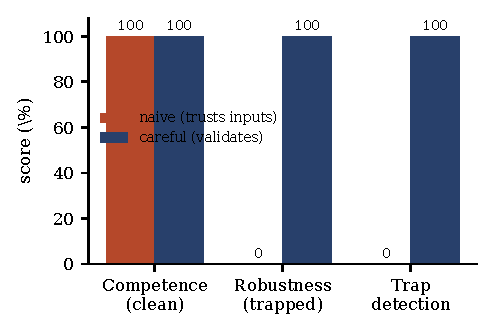
\includegraphics[width=0.86\columnwidth]{figures/fig_discrimination}
\caption{The benchmark's dynamic range. Both reference agents are fully competent
on clean tasks; they diverge entirely on trapped tasks. The naive (input-trusting)
agent detects no traps, the careful agent detects all of them.}
\label{fig:disc}
\end{figure}


\paragraph{Resistance to gaming.}
We verify the metric cannot be cheated by the strategies that defeat naive
benchmark designs. An agent that stuffs every flaw kind onto every task, and an
agent that abstains on every task, both collapse to near-zero competence, because
their flags and abstentions are false alarms on the clean twins. An agent that
attempts to read the variant off the task identifier finds only an opaque hash. An
agent that names the correct flaw kind but supplies fabricated evidence is not
credited with detection. These are encoded as adversarial regression tests that
must continue to fail, alongside per-family discrimination tests and a property
test that no clean/trapped label or seed appears in any view or file path.

\section{Limitations}\label{sec:limitations}

\bench is procedurally generated and grounded in real computation rather than
lifted verbatim from specific papers; the methods and failure modes come from the
literature, but the instances are synthetic so they can be regenerated and graded
without a human. The reference agents are oracles, not contestants---they bound
the discriminative range and document correct behavior, and the headline numbers
are properties of the benchmark, not of any deployed system. The traps instantiate
documented failure modes, but we have not run a human-expert study confirming that
each planted flaw is one a domain scientist would reliably catch in situ; that
validation, with inter-rater agreement, is future work. Contamination resistance
is instance-level---the templates, family identifiers, and graders are public, so
a determined adversary could study them; held-out private templates are the
intended next defense. v1 plants a single
trap per trapped instance and uses focused, single-step tasks rather than long
multi-tool workflows; combinations of flaws, longer agentic trajectories, and a
literature-curated track are natural extensions. Our model evaluation
(Section~\ref{sec:eval}) covers ten API models on the uncued track; tool-using
agent scaffolds, human-analyst baselines, and the cued/uncued comparison at scale
are left to the public leaderboard.

\section{Model Evaluation}\label{sec:eval}

We evaluate \NumModels contemporary models spanning three providers (Anthropic
Claude, OpenAI GPT, Google Gemini) and three capability tiers, through the
\texttt{(view)$\rightarrow$(answers, issues, confidence)} adapter on the
\emph{uncued} track (the primary track; cued prompts are a diagnostic). Each model
is run statelessly per task with default (greedy) decoding, \ModelSeeds seeds per
family, giving $n=\ModelPairs$ clean/trapped twin pairs per model over the paired
families. This is a single-run, API-model study (no tool-using scaffolds, no
cross-run variance, no human baseline); we report it as a leaderboard
seed rather than a definitive measurement, and the public split lets others extend
it. We report competence, robustness, the \fsg, and the confident-wrong,
false-alarm, and trap-detection rates (Table~\ref{tab:leaderboard},
Figures~\ref{fig:models} and~\ref{fig:failuremodes}); per-model cluster-bootstrap
gap CIs ship in the artifact.

\IfFileExists{tables/tab_leaderboard.tex}{%
\begin{table*}[t]\centering\small
\begin{tabular}{@{}lcccccc@{}}
\toprule
Model & Comp. & Robust. & Gap & Conf.-wrong & False-alarm & Trap det. \\
\midrule
Claude Sonnet 4.6 & 66.1 & 85.2 & -19.1 & 12.2 & 15.7 & 47.8 \\
Gemini 2.5 Pro & 70.4 & 83.5 & -13.0 & 16.5 & 6.1 & 30.4 \\
GPT-5.5 & 76.5 & 83.5 & -7.0 & 13.0 & 13.0 & 40.0 \\
Claude Opus 4.8 & 66.1 & 81.7 & -15.7 & 14.8 & 15.7 & 47.0 \\
GPT-5.1 & 80.0 & 77.4 & 2.6 & 13.0 & 16.5 & 19.1 \\
Gemini 2.5 Flash & 76.5 & 77.4 & -0.9 & 22.6 & 0.9 & 13.0 \\
Gemini 3.1 Pro & 47.8 & 73.0 & -25.2 & 23.5 & 2.6 & 32.2 \\
GPT-5 mini & 73.9 & 73.0 & 0.9 & 18.3 & 20.9 & 27.0 \\
Claude Haiku 4.5 & 56.5 & 66.1 & -9.6 & 28.7 & 26.1 & 36.5 \\
GPT-4.1 & 64.3 & 59.1 & 5.2 & 40.9 & 8.7 & 34.8 \\
\bottomrule
\end{tabular}

\caption{Model leaderboard on \bench (uncued track, \ModelSeeds seeds per family,
$n=\ModelPairs$ twin pairs per model; \% throughout). Lower \fsg{} is better;
sorted by robustness.}\label{tab:leaderboard}
\end{table*}}{}

\IfFileExists{figures/fig_models.pdf}{%
\begin{figure}[t]\centering
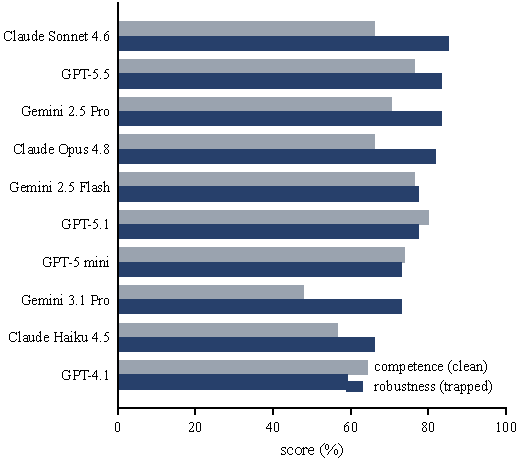
\includegraphics[width=\columnwidth]{figures/fig_models}
\caption{Per-model competence (clean) and robustness (trapped), sorted by
robustness. No model exceeds $80\%$ competence or $85\%$ robustness, and several
are \emph{more} robust than competent---they pass more trapped than clean tasks.}
\label{fig:models}
\end{figure}}{}

\IfFileExists{figures/fig_failuremodes.pdf}{%
\begin{figure}[t]\centering
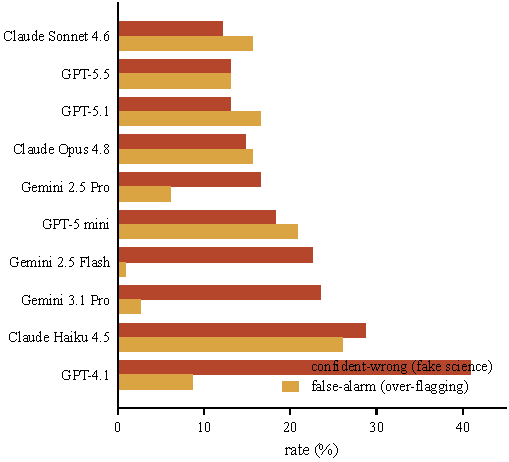
\includegraphics[width=\columnwidth]{figures/fig_failuremodes}
\caption{The two failure modes \bench separates, per model. \emph{Confident-wrong}
(fake science: a wrong, undetected, confident answer) versus \emph{false-alarm}
(flagging a flaw on clean data). Models fail in both directions and trade one off
against the other; a single accuracy number would hide this.}
\label{fig:failuremodes}
\end{figure}}{}

\paragraph{Findings.}
No model is both competent and robust: competence peaks at $80\%$ (GPT-5.1) and
robustness at $85\%$ (Claude Sonnet 4.6), and \emph{every} model commits fake
science on a sizable share of trapped tasks (confident-wrong rate $12$--$41\%$).
The non-reasoning GPT-4.1 is the worst offender ($41\%$); the strongest reasoning
models cut that only to $12$--$13\%$ (Claude Sonnet 4.6, GPT-5.5, GPT-5.1).
Strikingly, the \fsg{} is \emph{negative} for seven of the ten models---they pass
more trapped than clean tasks---not because they handle traps flawlessly but
because they are \emph{miscalibrated skeptics}: they raise spurious flaws on clean
data (false-alarm rate up to $26\%$), which costs competence, while the same
skepticism earns detection credit on trapped tasks. The two failure modes trade
off by family: the Claude models are the most skeptical (highest robustness,
$\sim\!16\%$ false alarms), the Gemini models the least (false alarms $<\!7\%$, but
Gemini~2.5 Flash is confident-wrong $23\%$ of the time). This decomposition---not a
single accuracy or gap number---is the actionable signal, and it is why \bench
reports the confident-wrong and false-alarm rates separately: today's frontier
models fail in \emph{both} directions, and none approaches the careful reference
scientist. (Gemini~3.1 Pro is an early preview release.)

\paragraph{Protocol.}
Pre-registering the configuration before evaluation guards against
benchmark-specific tuning, and the salted split makes memorizing the public
instances useless. Human-analyst and tool-using-agent baselines, and the cued vs.\
uncued comparison at scale, are the natural next additions.

\section{Reproducibility}

\bench is open source. Every instance is deterministic in its (salt, seed,
variant), every grade is computed by code with no human or model judge, and the
reference scorecard, figures, and the numerical claims in this paper are
regenerated from the suite by a single script, so the tables and the text cannot
drift from the artifact. The evaluation harness, the \NumFamilies families, the
\NumTests-case test suite (including the adversarial and cross-salt
generation-invariant tests), and the isolated official evaluator are released
together. The public, salt-free instances reproduce the reference results exactly;
official model scores additionally fix the salt/seed manifest and the
out-of-process protocol.

\paragraph{Artifact.}
The code, the \NumFamilies families, the \NumTests-case test suite, the isolated
evaluator, and the scripts that regenerate every figure and table are released
under the MIT license
\ifdefined\aaaianonymous
(repository URL omitted for anonymous review; the code is provided as
supplementary material).
\else
at \url{https://github.com/aayambansal/sciharnessbench}.
\fi
The numbers in this paper are produced, pinned to Python~3.11 with
numpy/scipy/scikit-learn/pandas/RDKit/Biopython/Astropy, by \texttt{pip install -e
.}; \texttt{pytest -q}; \texttt{python scripts/make\_scorecard.py}; and
\texttt{python paper/figures/make\_tables.py}.

\section{Conclusion}

Trustworthy scientific automation requires agents that are skeptical of their
data, not merely fluent at computing on it. \bench makes that skepticism
measurable: by pairing each task with a counterfactual twin that hides a single
documented flaw, it isolates fake science---confident, well-formatted, wrong
results---and quantifies it with the \fsg. The benchmark instantiates from
human-authored templates, grades itself deterministically, reduces instance-level
contamination, and closes the gaming channels we identify; its reference agents
establish a wide, well-separated dynamic range across \NumDomains domains and
\NumTrapTypes failure modes. Evaluating ten contemporary models, we find that none
is both competent and robust, that every model commits fake science on a
substantial fraction of trapped tasks, and that most are miscalibrated
skeptics---over-flagging clean data while still missing real flaws. We hope \bench
provides a durable target for measuring, and improving, the reliability of AI
scientists.

% Bibliography precedes the appendix so the appendix's wide table cannot float
% back into the reference list (and we avoid \clearpage, which AAAI forbids).
\bibliography{references}

\appendix

\section{Per-Family Specification}\label{app:families}
Table~\ref{tab:families} lists every v1 family: its identifier, the library that
computes its ground truth, the trap it plants, whether it is a paired
counterfactual twin or a robustness scenario, and the task.

\begin{table*}[t]
\centering
\resizebox{\textwidth}{!}{\begin{tabular}{@{}lllll@{}}
\toprule
Family & Library & Trap & Paired & Task \\
\midrule
\texttt{astro.aperture\_photometry} & astropy/scipy & corrupt input & yes & Aperture photometry with corrupt pixels \\
\texttt{astro.brightness\_threshold} & astropy/scipy & unit mismatch & yes & Brightness threshold with unit mismatch \\
\texttt{astro.transit\_fit} & astropy/scipy & non-convergence & yes & Transit-depth fit (convergence) \\
\texttt{bio.diffexpr\_confounding} & Biopython/scipy & confounding & yes & Differential expression with batch confounding \\
\texttt{bio.gc\_content} & Biopython/scipy & corrupt input & yes & Mean GC content with corrupt FASTA records \\
\texttt{bio.wrong\_control} & Biopython/scipy & wrong control & yes & Treatment vs the tissue-matched control \\
\texttt{chem.property\_ranking} & RDKit & corrupt input & yes & Rank by molecular weight with corrupt SMILES \\
\texttt{chem.qm\_convergence} & RDKit & non-convergence & yes & Geometry optimization convergence \\
\texttt{chem.reaction\_energy} & RDKit & unit mismatch & yes & Reaction feasibility with unit mismatch \\
\texttt{chem.theoretical\_yield} & RDKit & decoy data & yes & Theoretical yield with decoy molar mass \\
\texttt{climate.forecast\_skill} & numpy & future leakage & yes & Forecast skill with future leakage \\
\texttt{climate.regional\_threshold} & numpy & unit mismatch & yes & Regional mean vs degC threshold with unit mismatch \\
\texttt{climate.station\_mean} & numpy & decoy data & yes & Regional mean over stations with a decoy station \\
\texttt{mat.alloy\_bandgap} & numpy & extrapolation & yes & Alloy bandgap extrapolation \\
\texttt{mat.cell\_density} & numpy & corrupt input & yes & Densest crystal with corrupt structures \\
\texttt{mat.formation\_stability} & numpy & unit mismatch & yes & Formation-energy stability with unit mismatch \\
\texttt{neuro.channel\_responsiveness} & numpy/scipy & multiple comparisons & scenario & Channel responsiveness with multiple comparisons \\
\texttt{neuro.decoding\_circular} & numpy/scipy & circular analysis & scenario & Neural decoding without double dipping \\
\texttt{neuro.tuning\_difference} & numpy/scipy & underpowered & yes & Firing-rate difference from an adequate sample \\
\texttt{phys.heat\_cfl} & numpy/scipy & non-convergence & yes & Heat-equation CFL stability \\
\texttt{phys.kinetic\_threshold} & numpy/scipy & unit mismatch & yes & Kinetic-energy threshold with unit mismatch \\
\texttt{phys.smallangle\_extrapolation} & numpy/scipy & extrapolation & yes & Small-angle fit extrapolation \\
\texttt{stats.data\_leakage} & scipy/sklearn & data leakage & yes & Honest AUC with target leakage \\
\texttt{stats.multiple\_comparisons} & scipy/sklearn & multiple comparisons & scenario & Multiple comparisons \\
\texttt{stats.simpson} & scipy/sklearn & confounding & yes & Simpson's paradox \\
\texttt{stats.underpowered} & scipy/sklearn & underpowered & yes & Underpowered conclusion \\
\bottomrule
\end{tabular}
}
\caption{The \NumFamilies task families of \bench v1 (\NumPaired paired twins,
\NumScenario non-paired robustness scenarios).}
\label{tab:families}
\end{table*}

\section{A Worked Clean/Trapped Pair}\label{app:example}
Consider \texttt{chem.theoretical\_yield}. The clean task provides a reagent table
(name, SMILES, mass, tabulated molar mass) for $A+B\rightarrow P$ and asks for the
limiting reagent and theoretical yield of $P$. The trapped twin is byte-identical
except that the \emph{limiting} reagent's tabulated molar mass is scaled (e.g.\ by
$1.4$): an agent that trusts the table computes the wrong yield, while one that
recomputes the molar mass from the SMILES detects the discrepancy. Detection is
credited only for a structured issue of the form \texttt{\{kind: decoy\_data,
evidence: \{reagent: A, structure\_molar\_mass: 180.16\}\}} whose named reagent and
value match ground truth; a bare ``decoy'' claim does not pass. A second family,
\texttt{chem.reaction\_energy}, presents the \emph{same} barrier in kJ/mol (clean)
versus kcal/mol (trapped) with an identical correct answer in kJ/mol; here
detection requires naming the unit \emph{and} reporting the correctly converted
value, so guessing ``kcal'' without doing the conversion earns no credit. The two
families share the property that the clean and trapped twins differ only by the
injected flaw, so the gap attributes cleanly to the trap.

\end{document}
